% vim: spelllang=es

\chapter{Rust y Tremor}

\section{¿Qué es Rust?}\label{sec:rust}

Dado que Rust es un lenguaje de programación que tan solo anunció su primera
versión en 2015, aún no es conocido por muchos desarrolladores. Esta memoria no
requiere conocimientos previos sobre Rust. Sin embargo, la implementación en sí
y otras partes más avanzadas, como el Anexo~\ref{annex:abi} o el
Anexo~\ref{annex:covariance}, asumen una familiaridad con el lenguaje más
extensiva. Para esos casos, se recomienda consultar el Anexo~\ref{annex:rust},
que entra en mayor detalle sobre el lenguaje.

Rust es un lenguaje de programación de sistemas compilado y de propósito
general. Su objetivo es maximizar el rendimiento y la seguridad tanto en memoria
como en concurrencia y sin necesidad de un recolector de basura. Las garantías
de seguridad son comprobadas en tiempo de compilación gracias a un modelo
estricto de programación y a un sistema fuerte y estáticamente tipado. No
permite punteros nulos, referencias colgantes, ni condiciones de carrera ---
aunque sí fugas de memoria.

Proporciona control a bajo nivel, manteniendo una productividad cercana a
lenguajes de alto nivel. Dispone de programación funcional, genéricos,
inferencia de tipos y macros, entre otros. También tiene soporte integrado para
la programación asíncrona, un modelo de concurrencia que puede ejecutar
eficientemente una gran cantidad de tareas de entrada y salida. No obstante, es
posible ignorar explícitamente el modelo de memoria y concurrencia para casos
avanzados en los que se necesite control completo.

Los programas en Rust se diseñan basándose en la composición, en lugar del
polimorfismo convencional de Python o C++. Se puede conseguir la misma
flexibilidad mediante tipos estructurados y un mecanismo llamado \emph{traits},
similar a las interfaces de Java, pero más potentes.

El ecosistema básico de Rust es altamente cohesivo: incluye el sistema de
compilado y administrador de paquetes \emph{Cargo}, el \emph{formatter} de
código \emph{Rustfmt} y el \emph{linter} \emph{Clippy}. La instalación de estas
herramientas se suele gestionar con el programa \emph{rustup}.

\section{¿Qué es Tremor?}\label{sec:tremor}

Tremor es un \emph{sistema de procesado de eventos}, que consiste en ``el
monitorizado y análisis (procesado) de flujos de información (datos) sobre cosas
que pasan (eventos)''~\cite{luckham2011event}. Tremor fue creado como una
alternativa flexible y de alto rendimiento a herramientas como Logstash,
\namecite{telegraf} o \namecite{flink}, pero ha evolucionado para soportar casos
de uso más complejos. Al contrario que algunos de esos programas, Tremor también
tiene soporte para \emph{agregación} y \emph{rollups}, e incluye un lenguaje
\emph{ad hoc} para \emph{Extract, Transform, and Load} (ETL).

Para más información sobre Tremor se puede consultar \namecite{tremorintro}, que
introduce sus conceptos más básicos y sus posibles usos --- o cuándo \emph{no}
usarlo, en \namecite{tremorconstraints}. \namecite{tremorrecipes} lista un total
de 32 ejemplos de cómo configurar y emplear el software. El
Anexo~\ref{annex:tremor} explica el funcionamiento interno del programa.

\textcite{robins2010complex} y \textcite{cugola2012processing} introducen en
detalle los dos campos contenidos en Procesado de Eventos: \emph{Procesado de
Eventos Complejos} y \emph{Procesado de Flujos de
Eventos}\footnote{Siguiendo la terminología anglosajona, \emph{Complex Event
Processing} y \emph{Event Stream Processing}, respectivamente.}, ambos
relevantes a Tremor. \textcite{dayarathna2018recent} y
\textcite{tawsif2018review} resumen los avances más recientes en el campo,
analizan su evolución, y clasifican sus subáreas. La mayoría de la información
teórica tanto en esta sección como en el Anexo~\ref{annex:tremor} se extrae de
estas fuentes.

\subsection{Casos de uso}

La Figura~\ref{fig:tremor_example} ilustra uno de los casos de uso más básicos
de Tremor:

\begin{enumerate}
    \item Recibir \emph{logs} (eventos) de aplicaciones en diferentes protocolos
        o formatos. Es posible que esta heterogeneidad se deba a que algunas
        aplicaciones son legadas y no se puedan reducir a un único protocolo o
        formato, o que esta tarea es demasiado compleja como para gestionarse a
        nivel de aplicación.

    \item Filtrar los eventos redundantes, añadir campos nuevos o eliminar
        aquellos innecesarios y transformar todo a un mismo formato. El uso de
        una herramienta ineficiente o \emph{ad hoc} por la empresa podría ser
        inviable dada una cantidad de datos suficientemente grande o demasiados
        protocolos y formatos como para implementarlos todos.

    \item Enviar todos los logs estructurados a una base de datos u otras
        fuentes para analizarlos posteriormente.

\end{enumerate}

\begin{figure}
    \centering
    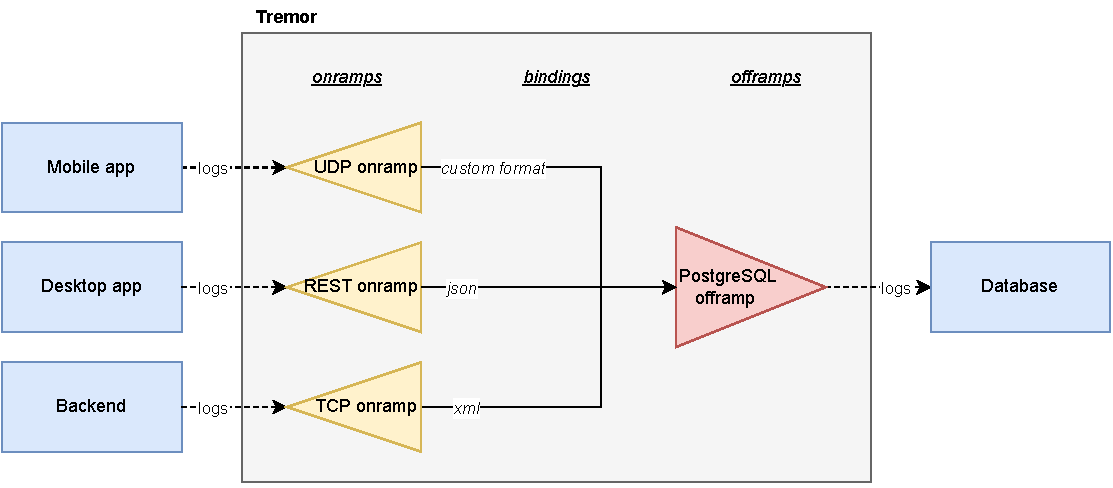
\includegraphics[width=\textwidth]{./Imagenes/example.pdf}
    \caption{Ejemplo de uso básico de Tremor}%
    \label{fig:tremor_example}
\end{figure}

Sin embargo, este caso subestima el potencial de Tremor. La entrada y salida del
sistema se pueden abstraer más, por ejemplo implementando un chatbot que
reproduce música. Este podría tomar mensajes de Discord como su entrada, y
enviar comandos con el API de Spotify como salida.

\subsection{Conceptos básicos}

Tremor se basa en los términos de \onramps o \sources y \offramps o \sinks:

\begin{itemize}
    \item Una \onramp especifica cómo Tremor se conecta con el mundo exterior (o
        una \pipeline) para \textbf{recibir} de sistemas externos. Por ejemplo
        TCP, periódicamente o PostgreSQL~\cite{tremoronramps}.

    \item Una \offramp especifica cómo Tremor se conecta con el mundo exterior
        (o una \pipeline) para \textbf{enviar} a sistemas externos. Por ejemplo,
        \emph{stdout}, Kafka o ElasticSearch~\cite{tremorofframps}.

    \item Una \pipeline es una serie de operaciones (transformación, agregación,
        eliminación, etc) a través de la cual se pueden encaminar los
        eventos~\cite{tremorpipelines}.

\end{itemize}

Estos \onramps u \offramps suelen contener una cantidad de información que es
demasiado grande como para guardarla y que debería tratarse en tiempo real. Su
procesado se basa en las siguientes operaciones:

\begin{itemize}
    \item \emph{Filtros}: descarte de eventos enteros a partir de reglas
        configuradas, con el objetivo de eliminar información de la \pipeline
        que no se considera relevante.

    \item \emph{Transformaciones}: conversión de los datos de un formato a otro,
        como por ejemplo incrementar un campo con un contador, reemplazar
        valores, o reorganizar su estructura.

    \item \emph{Matching}: búsqueda de partes de eventos que siguen un patrón en
        específico (por ejemplo, un campo \code{"id"} con un valor númerico)
        para transformarlo o descartarlo.

    \item \emph{Agregación} o \emph{rollups}: recolección de múltiples eventos
        para producir otros nuevos (como la media o el máximo de un campo), de
        forma que la información útil se reduzca en tamaño.

\end{itemize}

Finalmente, otros términos misceláneos sobre Tremor:

\begin{itemize}
    \item \emph{Códec}: describen cómo decodificar los datos del flujo y como
        volverlos a codificar. Por ejemplo, si los eventos de entrada usan JSON,
        tendrá que especificarse ese códec para que Tremor lo pueda entender.

    \item \emph{Preprocesador} o \emph{postprocesador}: operadores sobre flujos
        de datos brutos. Un preprocesador aplicará esta operación antes del
        códec y un postprocesador después. En particular, \code{base64} codifica
        o decodifica la información con ese protocolo.

    \item \emph{Artefacto}: término genérico para hablar de \sinks, \sources,
        códecs, preprocesadores y postprocesadores.

\end{itemize}

\subsection{Conectores}

Es posible que algunas \onramps no solo quieran recibir de sistemas externos,
sino también responderles directamente, actuando como una \offramp y viceversa.
Esto es especialmente útil para casos como REST y \websockets, donde el
protocolo da la posibilidad de responder a eventos usando la misma conexión, por
ejemplo con un ACK. En la versión 0.11 --- la presente cuando me uní al proyecto
--- este problema se solucionaba con el concepto de \emph{linked
transports}~\cite{tremorlinkedtransports}.

El término \emph{conector} se introdujo en mayo de 2022 con la versión
0.12~\cite{tremorconnectors}. Solucionan el problema desde el inicio,
abstrayendo tanto los \onramps como los \offramps bajo el mismo concepto,
incluyendo los \emph{linked transports}. Dado que estos ya estaban siendo
desarrollados mientras 0.11 era la última versión, el sistema de plugins se
enfocó a los conectores desde el principio, en lugar de \onramps u \offramps,
que ahora han quedado en desuso.
